\chapter{Style-based Tone mapping}
\label{chp:b4}

HDR image similarity has many applications, and one of these applications on tone mapping is presented in this chapter. The tone mapping operator that is depicted in the following sections named as style-based tone mapping, consists of a methodology that employs image similarity to tone map HDR images consistently according to a style without manual parameter adjustments. In this chapter, first the problem definition and the details of the method are given followed by the obtained tone mapping results.

\section{Problem Definition}

Tone mapping operators aim to reduce the dynamic range of an HDR image to display it on an low dynamic range display devices. The existence of numerous tone mapping operators that are available paved the way for many studies that are conducted for selecting the best one~\cite{parraga2018tone}. However, tone mapping can be conducted for different purposes, and rendering the resulting images to follow a consistent style can be one of them. For example, in a movie production process, making all frames consistently tone mapped, regardless of the content of the frames, can be a desired operation to impart a certain look and feel to the viewers. Although obtaining different renderings from tone mapping operators is partly achievable by using different tone mapping parameters, some tone mapping operators have none~\cite{Dura02} or few parameters~\cite{Fatt02} while others~\cite{Photomatix2010} have too many. Besides, even though one set of parameters are found for a certain image to depict a certain style of rendering, the same set of parameters would not yield with the same look when applied to other images. %that has different characteristics.

In this chapter, style based tone mapping operator that aims to consistently tone map different HDR images with the defined style is proposed. Figure \ref{fig:styles} shows different styles for the same images created by an artist. The application depicted in this thesis approaches the problem of defining a style by presenting the user an HDR image and with the help of the tool developed, ask the user to change the parameters until the image matches the desired look. By repeating this process for a small set of calibration images, we aim to \emph{learn} the style. Applying the learned style from calibration images to the previously unseen images is essentially a visual image similarity problem.

\begin{figure}
\begin{center}
\includegraphics[width=\textwidth]{figures/chapter5/styles.png}
\caption{Different artists may prefer different tone reproductions of the same HDR image. The same artist may also choose to produce different styles based on the situational/contextual considerations. The images reproduced by a professional artist using a different tool (top half) are replicated using our operator (bottom half). Presented algorithm can also learn the styles of an artist and produce results consistent with them.}
\label{fig:styles}
\end{center}
\end{figure}
%First, the problem of relating the input HDR image and the calibration images are solved with a method that has been commonly used for LDR images in the earlier work and then two different but related methods that uses the findings from the user experiment of visual similarity for HDR images discussed in Chapter \ref{chp:b3} and Chapter \ref{chp:b4} are employed.
%To summarize, the primary difference of the current method from the earlier work is its ability to learn about the various tone mapping styles that may be desired by an artist from a small set of calibration images. These styles can then be applied when tone mapping a new HDR image. Our algorithm is the first of its kind that gives the ability to batch process a large number of HDR images with respect to different styles.
\section{Method}
Style based tone mapping ~\cite{akyuz2013style} consists of two consecutive phases, namely \emph{calibration} and \emph{operation}. Calibration is the phase where the user defines a style and by manually adjusting the provided parameters tone maps a small set of images until the tone mapped image depicts the newly defined style. The next phase, operation is the phase that the user given HDR image is tone mapped automatically with the selected predefined style in the calibration phase by estimating the tone mapping parameters from the calibration image tone mapping parameters. Figure \ref{fig:calibration_operation} shows the style based tone mapping algorithm steps and these steps are explained in detail in the following sections.

\begin{figure}
\begin{center}
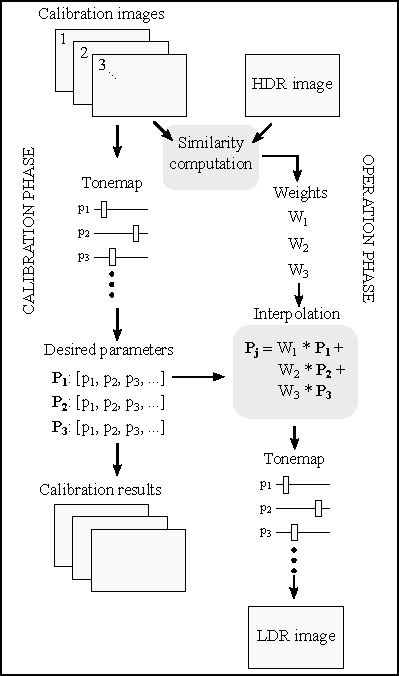
\includegraphics[width=0.65\textwidth]{figures/chapter5/algorithm.pdf}
\caption{Style based tone mapping is comprised of a calibration and operation phase. The artist tone maps several images during calibration which results in a set of parameters. During operation, these parameters are interpolated based on image similarity to find the tone mapping parameters for the given image.}
\label{fig:calibration_operation}
\end{center}
\end{figure}

\subsection{Calibration}
In the calibration phase, first the user is asked to pick a name for the new style to be created, and then the user is asked to tone map a fixed set of calibration images. Assigning a name to the style would be helpful for the user to stay consistent with the style while tone mapping the calibration images. In addition, once the style is created and saved, this will allow the user to have many predefined styles in preset library and reuse them. 

Calibration images should be representative enough for different environments that has different characteristics and at the same time distinctive from each other as much as possible to keep the number of the calibration images low. The number of calibration images directly affects the time spent in the calibration phase, so although more calibration images would represent different environments better, in order not to overwhelm the user, the number of calibration images is chosen in a way that the user can finish the calibration phase in a reasonable time.

Calibration images are selected in a semi automatic way. First, all images are taken from Fairchild's HDR image dataset~\cite{fairchild2007hdr} and then converted a feature space and using k-means algorithm each image in the dataset assigned to a cluster, which resulted in six clusters given in Appendix~\ref{app:clusters}. After clusters are obtained, one calibration image is hand-selected from each cluster, yielding six calibration images in total, which are shown in Figure \ref{fig:calibration_images}.

\begin{figure}
\begin{center}
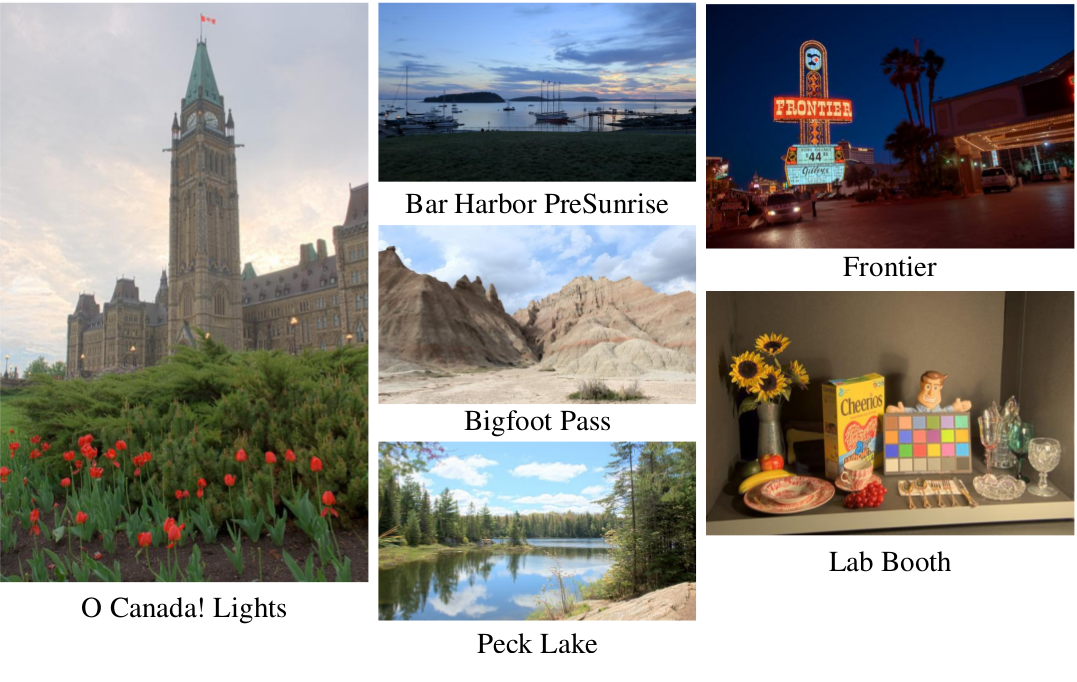
\includegraphics[width=\textwidth]{figures/chapter5/temp_calibration_images.png}
\caption{Calibration images
%paper
}
\label{fig:calibration_images}
\end{center}
\end{figure}

The calibration phase starts with naming the style, and then the user is presented with the tone mapping interface. With using this interface the user is required to tone map the calibration images one after another with the desired style. The manual tone mapping procedure is basically adjusting tone mapping parameters given in Table \ref{tab:tonemap_parameters} with the provided sliders.

\begin{table}
\caption{Tone mapping parameters for style-based tone mapping}
\label{tab:tonemap_parameters}
\centering
\begin{tabular}{|c|c|}
\hline 
Brightness ($b$) & Prct. mapped to half-max intensity \\
Contrast ($c$) & Slope of the tone curve at $b$ \\
Black point ($bp$) & Prct. clamped to min intensity \\
White point ($wp$) & Prct. clamped to max intensity \\
Color saturation ($c$) & Saturation control exponent \\
\hline
Small detail strength ($\lambda_s$) & UM factor for small details \\
Medium detail strength ($\lambda_m$) & UM factor for medium details \\
Large detail strength ($\lambda_l$) & UM factor for large details \\
\hline
\end{tabular}
\end{table}

The tone mapping operator is a modified version of Generic TMO~\cite{mantiuk2008modeling}. Generic TMO is able to model many existing tone mapping operators, both local and global with a tone curve followed by a spatial modulation function. It is noted in~\cite{mantiuk2008modeling} that same set of parameters yields very different results for different images. Style based tone mapping uses Generic TMO with the following modifications.

The tone mapping parameters of Generic TMO are replaced with their percentile counterparts in order to make the algorithm less image dependent and make it easier for user to have an understanding about the parameters. For example, the parameter \emph{Brightness} in style based tone mapping with the value 50 would correspond to the median brightness value of the HDR image in Generic TMO's \emph{b} parameter. Likewise, for the parameter \emph{White point}, the value 95 would mean 5\% of the brightest pixels will be burned out. As one may imagine, representing the tone mapping parameters as percentiles is not sufficient to achieve the same effect on different images. In order to achieve this, style based tone mapping uses parameter interpolation to use \emph{similar} parameters to \emph{similar} images as described in Section \ref{sec:operation}. 

The second modification to Generic TMO belongs to spatial modulation. In ~\cite{mantiuk2008modeling}, a linear combination of band-pass filters are used as spatial modulation function. These filters are from modified Cortex transform and applied after global tone curve modulation. On the other hand, in style based tone mapping, local modulation is applied in multiple scales and afterwards global operation is performed. This has the benefit of adjusting detail level before the HDR compression is applied and it gives better results. 

For detail modulation several approaches has been tested, unsharp masking (UM), bileteral filtering~\cite{Tomasi98} and gradient reversal removed BF~\cite{Bae2006}. While BF-based filters results with less halo, they are computationally expensive, unlike UM, which is prone to halos but computationally efficient. Besides, UM is shown to be improve sharpness and local contrast in an earlier study~\cite{Trenta2012}. It is decided to use UM even though it may introduce halos. For some cases, halos may be also introduced by the user in order to create an unrealistic style.

The detail modulation is achieved by first creating three low-pass images in the logarithmic domain for $small$, $medium$ and $large$ details.
\begin{align}
L'_{\sigma_s} &= g _{\sigma_s} * L', \\
L'_{\sigma_m} &= g _{\sigma_m} * L', \\
L'_{\sigma_l} &= g _{\sigma_l} * L', 
\end{align}
where $L' = log L$ and $g_\sigma$ are 2D Gaussian filters are different scales. $\sigma_s$, $\sigma_m$, and $\sigma_l$ are set to 0.0625\%, 0.3125\% and 0.625\% of the minimum image dimension respectively. Then these low pass images are used to enhance different scales with the chosen detail factor parameters $\lambda$.
\begin{equation}
    L_{sm} = e^{L' + \lambda_s(L' - L'_{\sigma_s}) + \lambda_m(L'_{\sigma_s} - L'_{\sigma_m}) + \lambda_l(L'_{\sigma_m} - L'_{\sigma_l})}
\end{equation}
$L_{sm}$, spatially modulated luminance image, then fitted to the tone curve as in~\cite{mantiuk2008modeling}. 

\begin{equation}
    TC(L_{sm}) = 
    \begin{cases}
    0 &\text{  if  $L_{sm}' \leq b - d_l$ } \\
    \frac{1}{2}c {{L_{sm}' - b}\over{1 - a_l(L_{sm}'-b)}} + \frac{1}{2} &\text{ if $b - d_l < L_{sm}' \leq b $ } \\ 
    \frac{1}{2}c {{L_{sm}' - b}\over{1 + a_h(L_{sm}'-b)}} + \frac{1}{2} &\text{ if $b < L_{sm}' \geq b + d_h$} \\ 
    1 &\text{ if  $L_{sm}' > b + d_h$}
    \end{cases}
\end{equation}

where $L_{sm}'$ is the logarithm of the spatially modulated luminance $c$ is the contrast, and parameters $b$, $d_l$ and $d_h$ are the absolute values of the user given parameters in percentiles for brightness, black point and white point respectively. Parameters $a_h$ and $a_l$ are contrast compression for light and dark areas computed from ~\cite{mantiuk2008modeling}.

\begin{equation}
    a_l = {{c . d_l-1} \over {d_l}} \text{ and } a_h = {{c . d_h-1} \over {d_h}}
\end{equation}

In Figure \ref{fig:calibration_phase}, the user interface that allows the user to define a style for tone mapping during the calibration phase is shown. The tone mapping parameters can be easily adjusted with the sliders and the calibration image will be tone mapped and shown to the user in real time. The luminance histograms of log HDR and LDR images are also shown to aid the user and show the effect of the changes. After all of the calibration images are tone mapped, the style parameters are saved and the calibration phase is completed. Manually stylized calibration images following the four styles presented in Figure~\ref{fig:styles} are given in Appendix~\ref{app:calib}.

\afterpage{
\begin{landscape}
\begin{figure}
\begin{center}
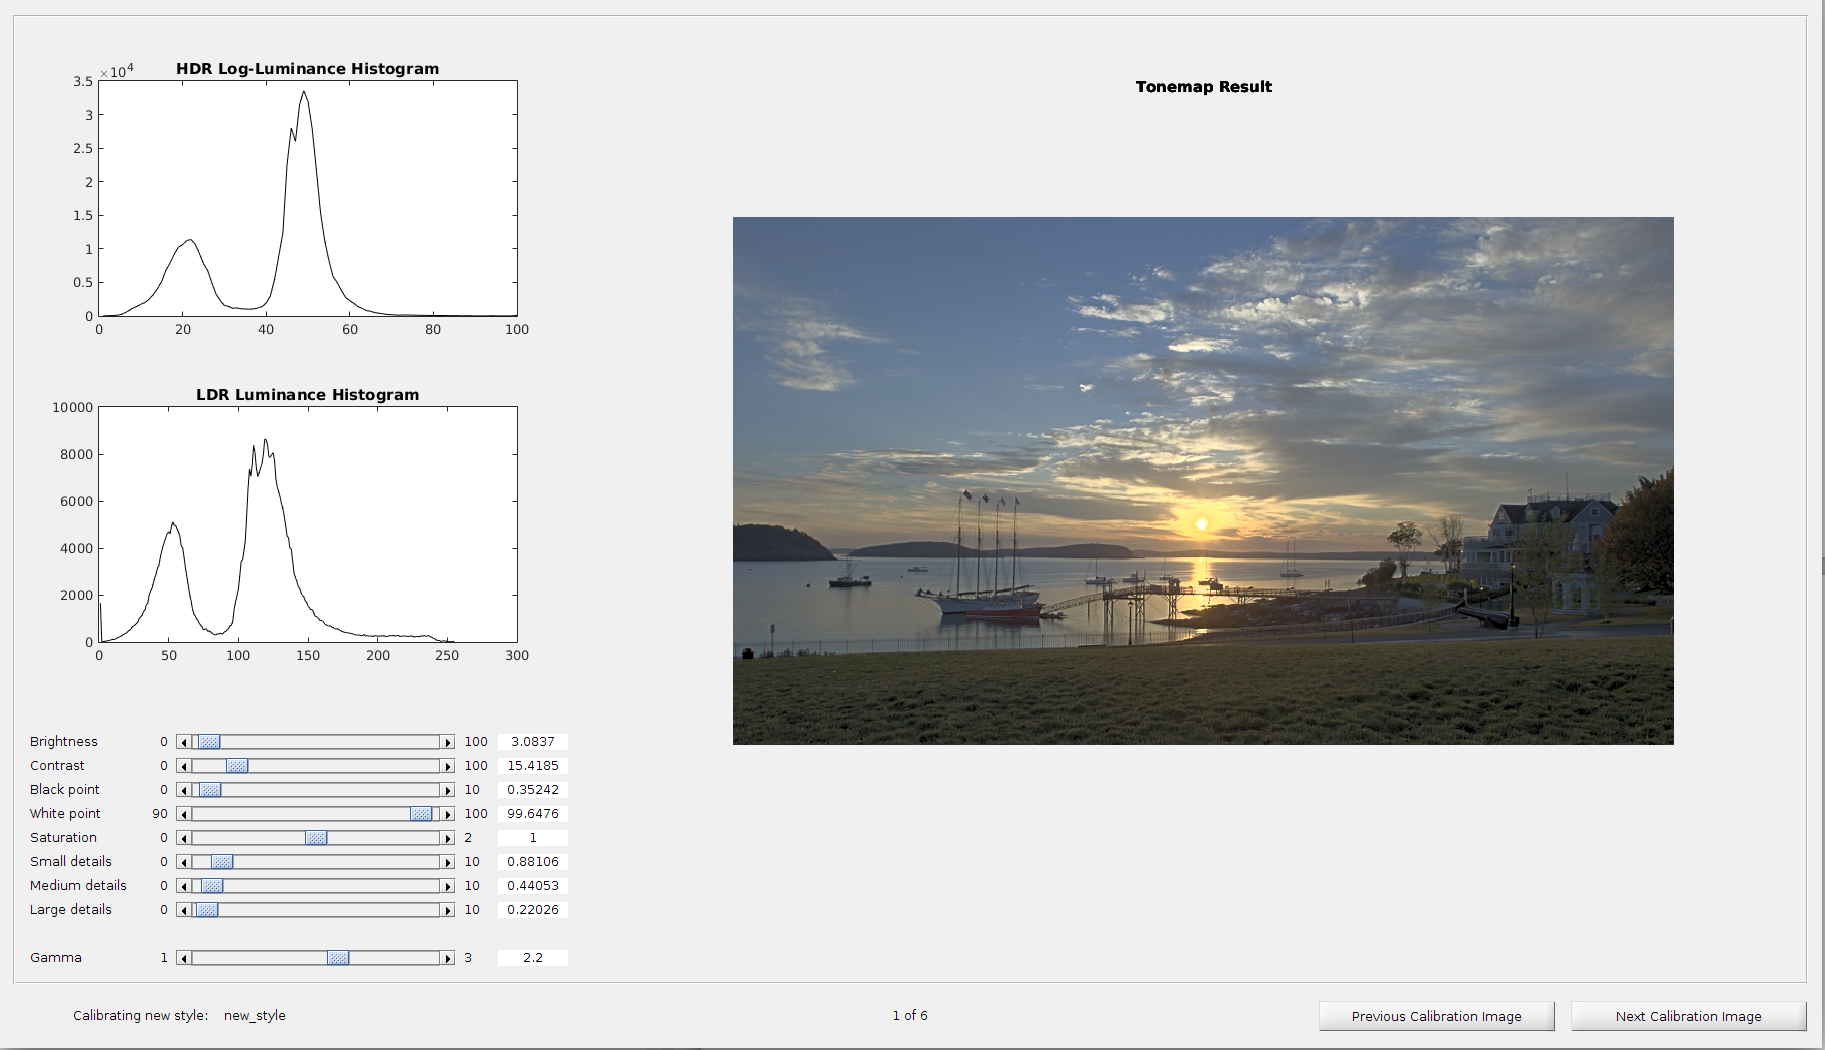
\includegraphics[height=0.85\textwidth]{figures/chapter5/ui_screenshot.png}
\caption{User interface for calibration phase}
\label{fig:calibration_phase}
\end{center}
\end{figure}
\end{landscape}
}

\subsection{Operation}
\label{sec:operation}
In the operation phase, the user selects a style from the preset library that has been created in the calibration phase. Given a new HDR image to be tone mapped with the selected style, the tone mapping parameters \emph{t} (given in Table \ref{tab:tonemap_parameters}) must be determined based on calibration images tone mapping parameters \emph{$t_i$}. In this thesis, this problem is approached as an image similarity problem. If two images are similar according to a similarity metric, their tone mapping parameters should be also similar. After the distances between input image and the calibration images are obtained, the tone mapping parameters are calculated as inverse distance transform~\cite{Shepard1968}:

\begin{equation}
\label{eq:inv_distance_transform}
    \mathbf{t} = {{\sum _{i=1} ^{N} {1 \over {d(\mathbf{f}, \mathbf{f_i})}} \mathbf{t_i}} \over {\sum _{i=1} ^{N} {1 \over {d(\mathbf{f}, \mathbf{f_i})}}}}
\end{equation}

Here, $\mathbf{f}$ is the feature vector of the current input image and $\mathbf{f_i}$ the feature vector for the calibration image $i$ and $\mathbf{t}$ its computed tone mapping parameters. Lastly, the function $d$ calculates the similarity between two feature vectors.

In~\cite{akyuz2013style}, images are represented with HSV histograms~\cite{Ben2006} and histograms of gradients~\cite{dalal2005histograms} to capture colorimetric and structural properties of the images. HDR images varies highly on pixel values and it is hard to compare them directly. To overcome this, images are tone mapped to the interval $[0,1]$:

\begin{equation}
    L_{out} = {{L_{in}} \over {1 + L_{in}}}, 
\end{equation}

and color channels are transformed with:

\begin{equation}
    \mathbf{C_{out}} = {{\mathbf{C_{in}}}\over{L_{in}}} L_{out}.
\end{equation}

The feature vector is then computed using transformed values, as a $60$ dimensional vector, $3x15$ bins for HSV histogram and $15$ bins for gradient histogram. 

Unfortunately, treating histograms as high dimensional points and computing their Euclidean distances does not yield correct results as this ignores the proximity information of the bins. For instance, although the histogram $H1 = (1, 0, 0, \cdots, 0)$ is closer to
$H2 = (0, 1, 0, \cdots, 0)$ than $H3 = (0, 0, 1, \cdots, 0)$, their Euclidean distances are equal. To circumvent this problem, each histogram is convolved with a 1-D Gaussian $(\sigma = 0.7)$ prior to computing their distances ~\cite{Ben2006}. Circular similarity of the hue histogram is also accounted. Thus the final distance metric between two feature vectors \textbf{$f_i$} and \textbf{$f_j$} become:
\begin{equation}
\label{eq:distance_metric}
    d(\mathbf{f_i, f_j}) = \mathbf{(f_i - f_j)}^T\mathbf{(f_i-f_j)},
\end{equation}

where \textbf{$f$} is the combined histogram. This metric is used to measure the similarity between input HDR image and calibration images. Also the same distance metric is used to cluster Fairchild dataset in order to pick calibration images.

After tone mapping parameters are calculated with parameter interpolation, HDR image is tone mapped and presented to the user in a similar user interface like Figure~\ref{fig:calibration_images}. User can do the final adjustments and save the tone mapped LDR image. Figure~\ref{fig:gallery} shows a gallery of the obtained tone mapping results. Note that despite the large variation of the image content, the selected styles are successfully applied to each image.

\begin{figure}
\begin{center}
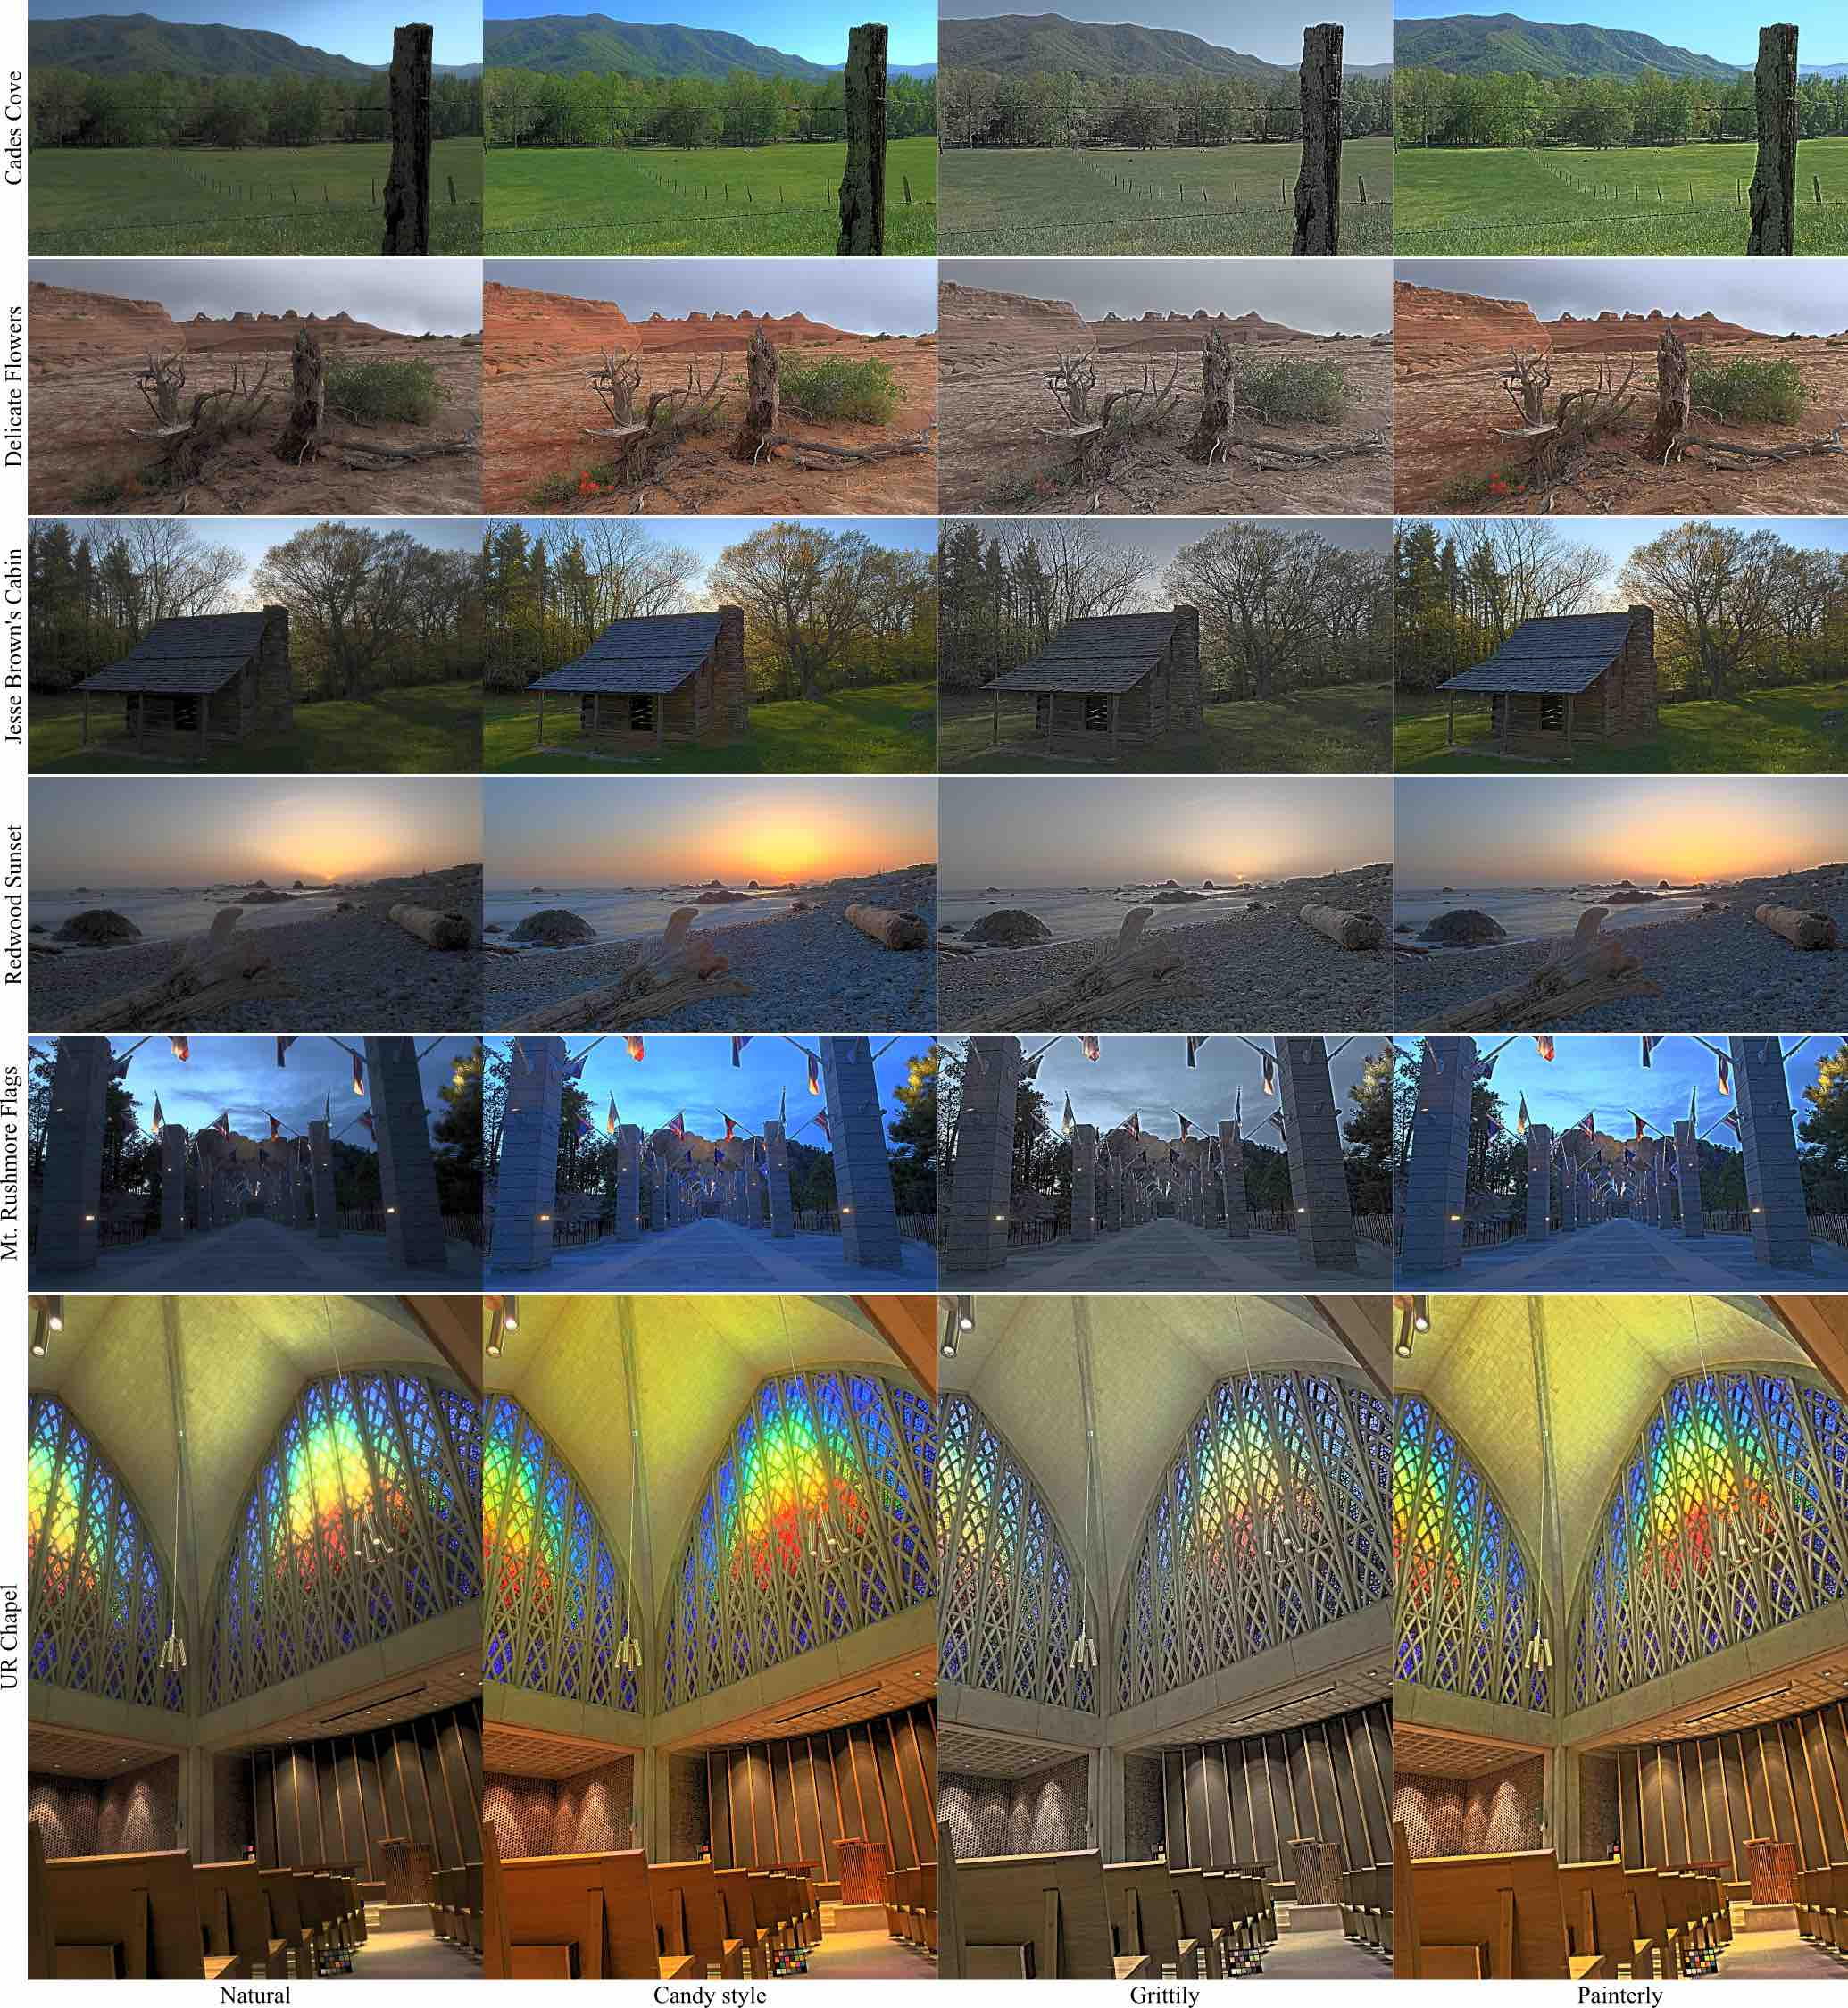
\includegraphics[width=\textwidth]{figures/chapter5/style_based/gallery_small.jpg}
\caption{All of these images are automatically tone mapped using the four styles that are generated.}
\label{fig:gallery}
\end{center}
\end{figure}

To sum up, tone mapping can be an artistic process that would result with different look and feel of the same scene instead of achieving a single "correct" look. The tone mapping methodology given in this chapter is versatile enough to create new styles with a small set of calibration images. And more importantly, with the leverage of image similarity, it is possible to apply the created styles to new HDR images automatically which can have quite different characteristics. However the similarity approach given in this chapter is rather straight forward and there is room for improvement. In the following chapters, two different similarity models backed up by a user study are suggested to improve style-based tone mapping.